\documentclass[a4paper, 12pt, oneside, onecolumn]{article}
\usepackage[utf8]{inputenc}
\usepackage[english]{babel}
\usepackage{geometry}
\usepackage{float}
\usepackage{graphicx}
\usepackage{amsmath}
\usepackage{amssymb}
\usepackage{lipsum}
\usepackage{systeme}
\usepackage{enumitem}
\usepackage{booktabs}
\usepackage{gensymb}
\usepackage{indentfirst}
\usepackage{esint}
\usepackage{harpoon}
\usepackage{relsize}
\usepackage{cite}
\usepackage{bm}
\usepackage{multicol}
\usepackage[useregional]{datetime2}
\usepackage[colorlinks = true, linkcolor = blue, hypertexnames = true]{hyperref}
\hypersetup{
    colorlinks=true,
    allcolors=blue	
}
\usepackage[super, square]{natbib}
\usepackage{epstopdf}
\usepackage{subfig}
\usepackage[subfigure]{tocloft}
\usepackage[affil-it]{authblk}
\usepackage{siunitx}


\newcommand{\cald}{{\rm d}}
\renewcommand\thesection{\Roman{section}}
\renewcommand{\thesubsection}{\thesection.\Roman{subsection}}
\renewcommand{\thesubsubsection}{\thesubsection.\Roman{subsubsection}}
\newcommand{\keywords}[1]{\textbf{Keywords:} #1}

\geometry{a4paper, scale = 0.90}
\linespread{1.5}
\setlength{\parindent}{2em}


\title{Explanation of the Mode II\\to Akantu Parameter Conversion Function}
\author[$\dagger$]{Gauss~T.~Chang}
\affil[$\dagger$]{Department of Civil Engineering, \url{R14521220@ntu.edu.tw}}
%\date{\DTMdate{2025-10-20}}
\date{\today}

\begin{document}
\maketitle

\section{Introduction}

In Akantu, cohesive elements are governed by a mixed-mode failure criterion.
However, in many experimental or theoretical studies, material properties are
obtained in pure Mode~II, such as the critical shear strength 
$\tau_{c}$ and the Mode~II fracture energy $G_{IIc}$. Akantu, in contrast, 
requires the following material parameters for its cohesive zone model:

\begin{itemize}
    \item $\sigma_{c}$ : the critical cohesive strength associated with the 
    mixed-mode effective stress criterion,
    \item $G_{c}$ : the fracture energy,
    \item $\beta$ : the mode-mixity parameter controlling the contribution of 
    shear in the failure criterion.
\end{itemize}

The Python function provided performs the conversion from the physically known
Mode~II quantities $(\tau_{c}, G_{IIc})$ into the parameters required by 
Akantu $(\sigma_{c}, G_{c}, \beta)$.

\section{Akantu Effective Stress Criterion}

Akantu defines an effective cohesive stress as
\begin{equation}
    \sigma_{\text{eff}}
    =\sqrt{\sigma_{n}^{2}+\frac{\tau^{2}}{\beta^{2}}},    
\end{equation}
where $\sigma_{n}$ is the normal traction and $\tau$ is the shear traction on 
the cohesive interface. Cohesive failure initiates when
\begin{equation}
    \sigma_{\text{eff}} > \sigma_{c}.
\end{equation}

\section{Specialization to Pure Mode II Loading}

For a pure Mode~II simulation, the opening stress is negligible,
$\sigma_{n}\approx 0$, so that the effective stress reduces to
\begin{equation}
    \sigma_{\text{eff}} = \frac{\tau}{\beta}.
\end{equation}

At the onset of failure,
\begin{equation}
    \sigma_{\text{eff}}=\sigma_{c},
\end{equation}
which implies:
\begin{equation}
    \frac{\tau_{c}}{\beta}=\sigma_{c}
    \qquad\Longleftrightarrow\qquad
    \sigma_{c}=\frac{\tau_{c}}{\beta}.
\end{equation}

Thus, the Akantu parameter $\sigma_{c}$ is directly computed from 
the desired Mode~II shear strength $\tau_{c}$ and the chosen mode-mixity
parameter $\beta$.

\section{Fracture Energy and Critical Shear Displacement}

In many cohesive zone formulations, including the bilinear model,
the Mode~II fracture energy is related to the critical shear 
displacement jump $\gamma_{c}$ through
\begin{equation}
    G_{IIc}=\frac{1}{2}\,\tau_{c}\,\gamma_{c}.
\end{equation}

Solving for $\gamma_{c}$ yields
\begin{equation}
    \gamma_{c}=\frac{2G_{IIc}}{\tau_{c}}.
\end{equation}

While Akantu does not require $\gamma_{c}$ as an input, it is computed 
in the Python function for consistency checking and for interpreting 
the physical scale of the cohesive separation.

\begin{figure}[H]
\centering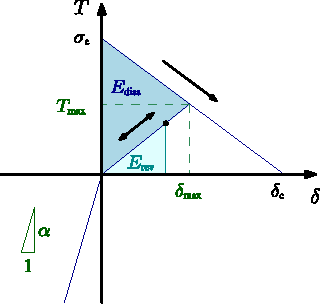
\includegraphics[height = 3in]{./linear_cohesive_law.pdf}
\caption{linear cohesive law.}\label{fig::Q1-d1}
\end{figure}

\newpage
\section{Function Summary and Interpretation}

The Python function converts Mode~II parameters to Akantu input parameters:
\begin{itemize}
    \item It computes $\sigma_{c} = \tau_{c}/\beta$, which is required 
    by Akantu's effective stress criterion.
    \item It sets $G_{c}=G_{IIc}$ for a pure Mode~II analysis.
    \item It computes $\gamma_{c}=2G_{IIc}/\tau_{c}$ for validation purposes.
    \item It returns $(\sigma_{c}, G_{c}, \beta, \gamma_{c})$ to be used in 
    the material definition.
\end{itemize}

The function therefore allows a user to select a small value of $\beta$
to suppress Mode~I failure and promote Mode~II behavior, while preserving 
the physically correct Mode~II fracture properties.

%\section{Python Code Referenced}
%
%\begin{verbatim}
%def convert_modeII_to_akantu(tau_c, G_IIc, beta):
%    """
%    Convert Mode II cohesive properties (tau_c, G_IIc)
%    into Akantu parameters (sigma_c, fracture energy, beta).
%    """
%
%    # sigma_c follows from tau_c = beta * sigma_c
%    sigma_c = tau_c / beta
%
%    # For pure Mode II, Akantu's fracture energy is simply G_IIc
%    G_c = G_IIc
%
%    # Bilinear CZM relation: G_IIc = 0.5 * tau_c * gamma_c
%    gamma_c = 2 * G_IIc / tau_c
%
%    return sigma_c, G_c, beta, gamma_c
%\end{verbatim}

\section{Conclusion}

The conversion procedure ensures that a user who possesses Mode~II cohesive 
properties can correctly construct an Akantu cohesive material model. The 
relationship $\sigma_{c}=\tau_{c}/\beta$ is essential for obtaining the desired 
shear-dominated failure behavior, especially when using a very small value of 
$\beta$ to suppress Mode~I failure.
\end{document}









\end{document}








































